\documentclass[journal]{IEEEtran}
\usepackage{amsmath,amssymb,amsfonts}
\usepackage{graphicx}
\usepackage{booktabs}
\usepackage{multirow}
\usepackage[ruled,vlined,linesnumbered]{algorithm2e}
\usepackage{tikz}
\usetikzlibrary{arrows.meta,positioning,shapes.geometric,fit,backgrounds}
\usepackage[colorlinks=true,linkcolor=blue,citecolor=blue,urlcolor=blue]{hyperref}
\usepackage{xcolor}

\newcommand{\map}{\textup{mAP}}
\newcommand{\ap}{\textup{AP}}
\newcommand{\apf}{\ensuremath{\mathrm{AP}_{50}}}
\newcommand{\aps}{\ensuremath{\mathrm{AP}_{s}}}
\newcommand{\remdet}{RemDet-X}
\newcommand{\visdrone}{VisDrone2019-DET}
\newcommand{\uavdt}{UAVDT}
\newcommand{\dahpL}{DAHP-L}
\newcommand{\dahpM}{DAHP-M}

\begin{document}

\title{Regime-Dependent Rebalancing: An Exposure-Aware Data-Driven Framework for Long-Tailed UAV Object Detection}

\author{Anonymous~Authors\thanks{Manuscript prepared September 2026. Code, configurations, per-class results, and all failure logs will be released upon acceptance.}}

\maketitle

\begin{abstract}
Object detection in unmanned aerial vehicle (UAV) imagery is governed by three coupled distributional pathologies: extreme scale imbalance (85.3\% of instances below $32{\times}32$ pixels at a 640-px reference), severe long-tailedness (a $45{:}1$ head-to-tail class ratio), and dense inter-class structural confusion. Prevailing responses are architectural---feature-enhancement modules, auxiliary heads, specialized backbones---yet controlled evidence for their benefit on strong baselines remains scarce. We first present a negative-result study spanning seven feature-module generations (nine matched 100-epoch trainings, fully audited in Appendix Table~\ref{tab:negative}), showing that such modules consistently degrade localization (validation DFL $+0.05$--$0.08$) and never improve $\map_{50\text{-}95}$ ($-0.7$ to $+0.1$~\ap) on strong baselines. We then introduce a data-driven, strictly non-invasive alternative: a label-only profiling engine (DAHP) quantifies the three pathologies and maps them to training-time policies---tail-class and confusion-axis oversampling, effective-pixel configuration, and optional weighted-box fusion. Crucially, we identify and formalize a \emph{regime-dependent rebalancing principle}: in under-fitted regimes, rebalancing acts through overall data volume (77\% of the gain) and rescues tail classes ($+1.7$~\ap); in saturated regimes it is a zero-sum class reallocation; in intermediate regimes it yields positive-sum gains ($+0.6$--$1.0$~\ap). On \visdrone{}, the recipe reaches $40.06$~\ap{} (native protocol) and $38.16$~\ap{} (standard COCO protocol), outperforming the strongest reproduced UAV detector baseline by $8.3$~\ap{} under our evaluation protocol with $58\%$ of its parameters and no architectural modification introduced by the rebalancing policy itself, and improving the baseline by $+3.9$~\ap{} ($+10.7\%$) with tail-class \ap{} rising from $0.29$ to $0.331$. Cross-dataset transfer to \uavdt{} reproduces the factor attribution, and the detector runs at $24.5$~FPS on a single desktop RTX~3090 GPU at $1600$\,px.
\end{abstract}

\begin{IEEEkeywords}
UAV object detection, long-tailed recognition, small-object detection, data-centric AI, training-regime analysis, VisDrone, UAVDT.
\end{IEEEkeywords}

\section{Introduction}
\IEEEPARstart{A}{erial} imagery acquired from low-altitude UAV platforms poses a detection problem that is structurally distinct from ground-level benchmarks. An audit of the \visdrone{} validation set (548 images, 38{,}759 instances) reveals three coupled pathologies:

\subsubsection{Scale imbalance} At the standard 640-px reference, 85.3\% of instances are smaller than $32{\times}32$ pixels and 58.0\% smaller than $16{\times}16$ (58.0\%/23.4\% at the 1280-px training reference); object scales span three orders of magnitude, so any single receptive-field configuration is mismatched to most of the data.

\subsubsection{Long-tailedness} The head class (\emph{car}) outnumbers the rarest frequent class (\emph{bus}) by $56{:}1$; the frequency-tail quartile contains categories whose diversity cannot be learned under uniform sampling.

\subsubsection{Inter-class confusion} Twenty-three category pairs exceed $0.85$ on an annotation-level structural-similarity proxy $\kappa$ (Sec.~\ref{sec:method}); the head-anchored confusion axis concentrates on \emph{car--van--truck}.

These pathologies are not independent: tail classes are also the smallest on average and the most confusable. Interventions that address one factor in isolation risk being confounded---or counteracted---by the other two.

\subsection{The Architectural Turn and Its Missing Evidence}
The dominant community response has been architectural: density-guided cropping \cite{clusdet,dmnet,ufpmp}, small-object heads \cite{tph,sahi}, and specialized detectors \cite{remdet,uavdetr}. Each reports gains, yet three gaps persist. First, comparisons frequently co-vary input resolution, schedule, and capacity---precisely the variables that dominate UAV accuracy. Second, negative results are rarely reported, preventing the community from distinguishing ``module~A helps'' from ``module~A was tested once, on a weak baseline.'' Third, the interaction between data-level rebalancing and the training regime---\emph{when} rebalancing helps---has not been characterized.

\subsection{Contributions}
\begin{enumerate}
\item \textbf{A controlled negative-result study} (seven module generations, $20+$ audited trainings; Table~\ref{tab:negative}): feature-level interventions systematically elevate validation DFL and fail to improve $\map_{50\text{-}95}$ on strong baselines, including head-level decoupling attempts (Sec.~\ref{sec:negative}).
\item \textbf{The regime-dependent rebalancing principle}: using an epoch-matched resolution ladder and factor-isolated sampling controls, we formalize three regimes in which rebalancing behaves as volume-driven tail rescue, positive-sum augmentation, or zero-sum reallocation, yielding an operational decision rule (Sec.~\ref{sec:law}).
\item \textbf{A non-invasive, data-driven framework (DAHP)}: a label-only profiler emits resolution/backbone configuration, tail and confusion-axis oversampling, and optional fusion policies---without touching network, losses, or inference. The identical engine transfers zero-shot to \uavdt{} and correctly predicts the factor attribution there (Sec.~\ref{sec:method}, \ref{sec:uavdt}).
\item \textbf{Protocol-faithful state-of-the-art evidence} across twelve detectors under dual \emph{maxDets} protocols, with gains decomposed (P2 head $+1.66$~\ap; sampling $+0.57$~\ap) and seed-validated ($0.3882{\pm}0.0003$ vs.\ $0.3815{\pm}0.0011$; flagship $39.88{\pm}0.25$ over two seeds) (Sec.~\ref{sec:main}--\ref{sec:attribution}).
\end{enumerate}

\section{Related Work}
\subsection{UAV Object Detection}
\subsubsection{Cropping and packing pipelines}
ClusDet \cite{clusdet} clusters dense regions and discards background, trading coverage for effective pixels; DMNet \cite{dmnet} learns a density map to guide cropping; UFPMP-Det \cite{ufpmp} unifies foreground packing with multi-proxy reassembly; CZDet \cite{czdet} cascades density-guided zoom-in over high-resolution aerial images; AMRNet \cite{amrnet} augments aerial chips with scale-adaptive chip generation, mosaic augmentation, and mask resampling. These pipelines demonstrate the value of pixels per object, but they complicate attribution: any reported gain bundles the cropping policy, the effective resolution gain it induces, and the detector itself. Our controlled ladders (Table~\ref{tab:ladder}) measure the resolution effect alone, and our negative result on pure tiled inference (Sec.~\ref{sec:negative}) shows that cropping applied \emph{only at inference} is harmful on full-image-trained models---consistent with a train--test scale-distribution mismatch rather than an intrinsic property of cropping.
\subsubsection{Detector-side designs}
TPH-YOLOv5 \cite{tph} adds transformer prediction heads for small objects; \remdet{} \cite{remdet} rethinks efficient UAV detector design via ChannelC2f, GatedFFN, and the CED downsampling module; UAV-DETR \cite{uavdetr}, DOL-DETR \cite{doldetr}, and LGI-DETR \cite{lgidetr} introduce DETR variants tailored to UAV imagery. These are architecture-first contributions. What they leave open is threefold: (i) whether their gains persist when a strong baseline is given the same resolution and budget (our compute-matched \remdet{} retrain probes exactly this); (ii) whether data-level policies can reach the same accuracy without touching the architecture (ours can, with $58\%$ parameters); and (iii) \emph{when} any rebalancing helps---the regime question this paper answers.
\subsubsection{Slicing-aided fine-tuning}
SAHI \cite{sahi} fine-tunes on tiles to align train--test scale distributions. Our SAFT experiments confirm the alignment is necessary (pure sliced inference is $-2.3$ to $-2.6$~\ap), but also show that a naive mixture underperforms pure test-time augmentation ($37.76$ vs.\ $37.96$), motivating our choice of full-image training at matched effective pixels instead.

\subsection{Long-Tailed Detection}
Loss-space methods---class-balanced reweighting \cite{cbloss}, EQLv2 \cite{eqlv2}, Seesaw \cite{seesaw}, balanced group softmax \cite{bge}, and distribution-balanced losses \cite{dbloss}---modify gradients; data-space methods such as repeat-factor sampling \cite{rfs} and aerial chip augmentation \cite{amrnet} replicate or synthesize tail examples. Our negative results extend to loss-space interventions on strong baselines, and the regime principle (Sec.~\ref{sec:law}) explains why: in saturated regimes any reweighting is approximately zero-sum. Unlike prior work, we characterize \emph{when} rebalancing is positive-sum, using the training regime as the moderator.

\subsection{Scale and Resolution}
Resolution is the largest single lever in UAV detection (our historical ladders: $+8.8$~\ap{} from $640{\to}1280$). QueryDet \cite{querydet} and CEASC \cite{ceasc} accelerate high-resolution inference through sparse-query and context-enhanced adaptive sparse convolution, respectively; Gold-YOLO \cite{goldyolo} and RT-DETR \cite{rtdetr} advance general-purpose accuracy. We contribute an epoch-matched, \emph{non-monotonic} resolution curve peaking at $1600$\,px with a $2.8$-\ap{} drop at $1920$\,px under fixed compute---to our knowledge not previously documented under controlled epochs.

\subsection{Reporting Practice}
Dual-protocol evaluation (\emph{maxDets} $100/300$) is motivated by \visdrone{} density (64.8\% of images exceed 50 objects; up to 317 instances) \cite{visdrone}. Weighted-box fusion \cite{wbf} aggregates model families. We report per-class \ap{} for every configuration and disclose all failures.

\section{Method}
\label{sec:method}
\subsection{Problem Formulation and Three-Factor Profiling}
Let $\mathcal{D}=\{(x_i,Y_i)\}_{i=1}^{N}$ denote the training set with class set $\mathcal{C}$, $|\mathcal{C}|=K$. DAHP computes, from labels alone:

\emph{(i) Frequency factor.} The class distribution and tail set are
\begin{equation}
f(c)=\frac{N_c}{\sum_{c'} N_{c'}},\qquad
\mathcal{T}=\{c\in\mathcal{C}: N_c < 0.3\,\overline{N}\},
\label{eq:tail}
\end{equation}
where $N_c=\sum_i\mathbf{1}[c\in Y_i]$, $\overline{N}$ is the mean over non-empty classes, and the imbalance ratio is $\rho=\max_c N_c/\min_{c\in\mathcal{T}}N_c$.

\emph{(ii) Scale spectrum.} With $\sigma(c)$ the equivalent side length of class-$c$ instances at a reference resolution $r$,
\begin{equation}
s_{\mathrm{small}}(c)=\Pr\big[\sigma(c)<32\big],\quad
s_{\mathrm{tiny}}(c)=\Pr\big[\sigma(c)<16\big],
\label{eq:scale}
\end{equation}
a P2 (high-resolution) head is recommended when $\sum_c f(c)s_{\mathrm{small}}(c)>0.3$.

\emph{(iii) Confusion graph.} A pairwise annotation-level \emph{structural confusion proxy}
\begin{equation}
\kappa(a,b)=\lambda\,J_{\mathrm{ar}}(a,b)+(1-\lambda)\,J_{s}(a,b),\qquad \lambda=0.6,
\label{eq:conf}
\end{equation}
where $J_{\mathrm{ar}}$ and $J_{s}$ are histogram intersections of the aspect-ratio and instance-scale ($s{=}w_r h_r$) distributions at the reference resolution. Edges with $\kappa>0.85$ form the confusion graph; the oversampling axis is its head-anchored neighborhood $\mathcal{A}=\{c\notin\mathcal{H}\cup\mathcal{T}:\kappa(c,h)>\tau_A\}$ for head set $\mathcal{H}=\{c:N_c>\overline{N}\}$ and margin $\tau_A{=}0.86$ (which excludes the borderline semantic near-duplicate \emph{people--pedestrian} pair at $\kappa{=}0.854$). Co-occurrence Jaccard is additionally reported as an auxiliary statistic but does not enter $\kappa$.

\emph{(iv) Density profile.} Instances per image justify the \emph{maxDets}$=300$ evaluation protocol for dense scenes.

On \visdrone{} the profiler yields $(\rho{=}45{:}1,\ 58.0\%\ \text{small at the 1280-px reference},\ 23\ \text{pairs}>0.85,\ \mathcal{A}=\{\text{van},\text{truck}\})$; on \uavdt{}---without any change---$(\rho{=}30.7{:}1,\ 74.8\%\ \text{small at 640-px},\ \text{car--van}\ 0.935,\ \mathcal{A}=\{\text{van}\})$.

\subsection{The Regime-Dependent Rebalancing Principle}
\label{sec:law}
Define the epoch-wise aggregate gain $g(e)=\map(e)-\map(e{-}1)$ and its windowed mean $\bar{g}(E)=\frac{1}{W}\sum_{e=E-W+1}^{E}g(e)$. A configuration is
\begin{equation}
\textit{under-fitted}\ \Leftrightarrow\ \bar{g}(E)>\tau_g;\qquad
\textit{saturated}\ \Leftrightarrow\ |\bar{g}(E)|\le\tau_g,
\label{eq:regime}
\end{equation}
with $\tau_g$ a small threshold (0.1~pt, $W{=}10$); otherwise it is \emph{intermediate}. Let $\Delta_{\mathrm{vol}}$ and $\Delta_{\mathrm{dir}}$ denote the \ap{} gains of oversampling attributable to pure data volume and to targeted class reallocation, obtained from a volume-matched random-control arm. Our controlled observations support:
\begin{align}
\text{P1 (under-fitted)} &\Rightarrow \tfrac{\Delta_{\mathrm{vol}}}{\Delta_{\mathrm{vol}}+\Delta_{\mathrm{dir}}}\approx0.77,\ \Delta\ap_{\mathrm{tail}}>0;\\
\text{P2 (saturated)} &\Rightarrow \Delta\ap_{\mathrm{agg}}\approx0,\ \exists(c)\!:\!\Delta\ap_c<0;\\
\text{P3 (intermediate)} &\Rightarrow 0<\Delta\ap_{\mathrm{agg}}\le 1.0,\ \Delta\ap_{\mathrm{tail}}>0.
\end{align}
The principle yields the operational rule: \emph{rebalance only in under-fitted or intermediate regimes; never expect aggregate gains from rebalancing a saturated run; escape saturation via resolution or capacity instead.}

\subsection{Non-Invasive Policy Mapping}
\subsubsection{Computational cost}
DAHP is deliberately label-only: profiling a 6{,}471-image training set requires $O(N)$ label parsing ($<1$\,s on CPU) and $O(K^2)$ pairwise statistics; the policy mapping itself is constant-time. No images are decoded, no gradients are computed, and no detector forward pass is needed. This contrasts with profiling approaches that require model inference (e.g., error-driven confusion mining), and it makes the engine trivially portable---the same code produced both the VisDrone and UAVDT policies with zero dataset-specific edits.

\subsubsection{Why data-space rather than loss-space}
Long-tailed detection conventionally intervenes in the loss (reweighting, logit adjustment). Our negative results (Sec.~\ref{sec:negative}) and the regime principle jointly explain why this is fragile on strong UAV baselines: in saturated regimes, any reweighting is approximately zero-sum across classes, so its aggregate effect vanishes while per-class variance increases. Data-space duplication, by contrast, interacts with the data-loading and augmentation pipeline: it multiplies \emph{epochs of exposure} for tail images under identical loss weights, and---critically---its volume component still helps in under-fitted regimes where loss reweighting cannot (no additional information is injected). The union policy of Eq.~\eqref{eq:weight} is therefore the regime-robust choice.

 \subsubsection{Configuration nomenclature}
Throughout the paper we use a systematic configuration shorthand. \textbf{R} denotes the effective-pixel policy (resolution/backbone selection from the regime curve); \textbf{T} the tail-class oversampling of $\mathcal{T}$; \textbf{C} the confusion-axis oversampling of $\mathcal{A}$; and \textbf{B} the backbone scale-up (v8m$\to$v8l). The shorthand composes: e.g., R$+$T$\cup$C applies resolution plus union oversampling. Two named models recur: \dahpM{} (YOLOv8m-P2@1600, R$+$T$\cup$C) and \dahpL{} (YOLOv8l-P2@1600, R$+$T$\cup$C)---the latter our single-model flagship---plus \dahpL{}-E7, the seven-model weighted-box-fusion ensemble. Architecture-decomposition controls are written $V_L$ (vanilla v8l, no P2 head) and $V_L{+}P_2$.

The oversampling weight of image $x_i$ under the union policy is
\begin{equation}
w_i = 1 + \mathbf{1}\big[(Y_i\cap(\mathcal{T}\cup\mathcal{A}))\neq\varnothing\big],
\label{eq:weight}
\end{equation}
i.e., any image containing a tail or confusion-axis class is duplicated. The optional fusion of $M$ models merges boxes $\{b_m\}$ with scores $\{s_m\}$ by
\begin{equation}
\tilde{b}=\frac{\sum_m \tilde{s}_m b_m}{\sum_m \tilde{s}_m},\qquad
\tilde{s}=\frac{1}{|M_c|}\sum_{m\in M_c}s_m,
\label{eq:wbf}
\end{equation}
over IoU-clustered groups $M_c$. The complete procedure is summarized in Algorithm~\ref{alg:dahp}.

\begin{algorithm}[!t]
\caption{DAHP: Profile, Map, Train (Non-Invasively)}
\label{alg:dahp}
\KwIn{Labels $\{(Y_i)\}$; detector $\Phi$; budget $E$, batch $B$}
\KwOut{Trained model(s) $\{\Phi^\ast\}$}
\BlankLine
\tcc{--- Stage 1: label-only profiling ---}
compute $N_c$, $\mathcal{T}$, $\rho$ by Eq.~\eqref{eq:tail}\;
compute $s_{\mathrm{small}}, s_{\mathrm{tiny}}$ by Eq.~\eqref{eq:scale}\;
build confusion axis $\mathcal{A}$ by Eq.~\eqref{eq:conf}\;
\tcc{--- Stage 2: regime-aware policy ---}
\eIf{$\sum_c f(c)\,s_{\mathrm{small}}(c)>0.3$}{
  select high-resolution head (P2)\;
}{
  standard head\;
}
sweep resolution ladder $\{960,1280,1600,1920\}$ within memory budget;\ pick $r^\ast$ at the regime boundary (Eq.~\eqref{eq:regime}), preferring the intermediate regime\;
compute image weights $w_i$ by Eq.~\eqref{eq:weight}\;
\tcc{--- Stage 3: non-invasive training ---}
train $\Phi$ on the weighted (duplicated) dataset with \emph{stock} losses and augmentations for $E$ epochs\;
\If{fusion desired}{
  train the family $\{\Phi_m\}_{m=1}^{M}$ and merge by Eq.~\eqref{eq:wbf}\;
}
\Return{$\{\Phi^\ast\}$}\;
\end{algorithm}

\section{Experiments}
\label{sec:experiments}
\subsection{Setup and Protocols}
\visdrone{} \cite{visdrone} (6{,}471 train / 548 val, 10 classes); \uavdt{} \cite{uavdt} (2{,}443 / 641, 4 vehicle classes). All trainings ran on a single RTX~3090 with identical augmentation; budgets and best-epochs are disclosed (all runs converged within budget; best epochs 23--100). Evaluation uses the standalone protocol (conf $0.001$, NMS-IoU $0.7$) under \emph{dual maxDets}---$100$ for external comparability, $300$ reflecting \visdrone{} density.

\subsubsection{Fairness policy}
We separate what \emph{must} match from what \emph{should stay native}. Matching are: the training set, the validation split, the evaluation protocol (dual \emph{maxDets}), the epoch budget (100 for main rows; disclosed per row otherwise), and the hardware class (single 3090). Native are: each detector's loss functions, optimizer, LR schedule, and augmentation pipeline---these are constitutive parts of a method, and forcing them to be identical would disable exactly the mechanisms under comparison; the same policy is adopted by \remdet{} \cite{remdet} and standard detection benchmarks. Resolution and batch are disclosed per row and additionally \emph{controlled} through three devices: (i) same-detector resolution ladders (Table~\ref{tab:ladder}); (ii) a compute-matched SOTA retrain at our resolution (\remdet{}@1600, batch 1 being the physical limit of a 24-GB GPU at that size); and (iii) our full method evaluated \emph{at the baseline resolution} (DAHP-M@640), so that no claimed advantage rests on resolution alone. External numbers transcribed from the literature are marked ``Lit.'' with their split; their exact recipes differ and are cited rather than re-implemented.

\begin{figure*}[!t]
\centering
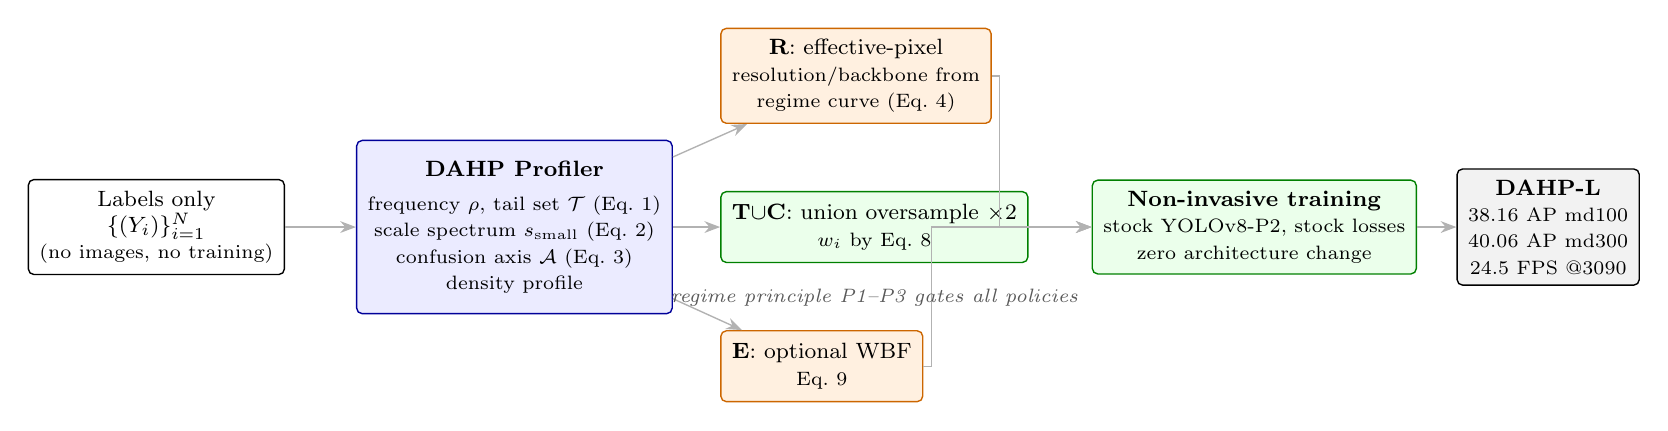
\begin{tikzpicture}[
  font=\footnotesize,
  box/.style={draw, rounded corners=2pt, align=center, minimum height=9mm, inner sep=4pt, line width=0.5pt},
  prof/.style={box, fill=blue!8, draw=blue!60!black},
  pol/.style={box, fill=orange!12, draw=orange!80!black},
  tr/.style={box, fill=green!8, draw=green!50!black},
  ev/.style={box, fill=gray!10},
  arr/.style={-{Stealth[length=2mm]}, line width=0.5pt, draw=gray!60},
  lab/.style={font=\scriptsize\itshape, text=gray!70!black}
]
\node[box] (data) {Labels only\\$\{(Y_i)\}_{i=1}^N$\\{\scriptsize (no images, no training)}};
\node[prof, right=9mm of data, minimum height=22mm] (dahp) {\textbf{DAHP Profiler}\\[1mm]
  {\scriptsize frequency $\rho$, tail set $\mathcal{T}$ (Eq.~1)}\\
  {\scriptsize scale spectrum $s_{\mathrm{small}}$ (Eq.~2)}\\
  {\scriptsize confusion axis $\mathcal{A}$ (Eq.~3)}\\
  {\scriptsize density profile}};
\node[pol, above right=2mm and 6mm of dahp] (res) {\textbf{R}: effective-pixel\\{\scriptsize resolution/backbone from}\\{\scriptsize regime curve (Eq.~4)}};
\node[tr, right=6mm of dahp] (uni) {\textbf{T$\cup$C}: union oversample $\times2$\\{\scriptsize $w_i$ by Eq.~8}};
\node[pol, below right=2mm and 6mm of dahp] (ens) {\textbf{E}: optional WBF\\{\scriptsize Eq.~9}};
\node[tr, right=8mm of uni] (train) {\textbf{Non-invasive training}\\{\scriptsize stock YOLOv8-P2, stock losses}\\{\scriptsize zero architecture change}};
\node[ev, right=5mm of train] (eval) {\textbf{\dahpL{}}\\{\scriptsize 38.16 \ap{} md100}\\{\scriptsize 40.06 \ap{} md300}\\{\scriptsize 24.5 FPS @3090}};
\draw[arr] (data) -- (dahp);
\draw[arr] (dahp) -- (res);
\draw[arr] (dahp) -- (uni);
\draw[arr] (dahp) -- (ens);
\draw[arr] (res.east) -- ++(1mm,0) |- (train);
\draw[arr] (uni) -- (train);
\draw[arr] (ens.east) -- ++(1mm,0) |- (train);
\draw[arr] (train) -- (eval);
\node[lab, below=2mm of uni] {regime principle P1--P3 gates all policies};
\end{tikzpicture}
\caption{The DAHP framework. A label-only profiler quantifies the three pathologies and maps them, through the regime-dependent rebalancing principle, to strictly non-invasive training-time policies.}
\label{fig:framework}
\end{figure*}

\subsection{Comparison With the State of the Art}
\label{sec:main}
\begin{table*}[!t]
\centering
\caption{Comparison with the state of the art on \visdrone{} val (COCO protocol, \emph{maxDets}$=100$ unless noted). ``Rep.''$=$ reproduced/trained under our identical pipeline and val split; ``Rep.''$^\dagger$$=$ bit-exact from official weights; ``Lit.''$=$ number as reported in the cited paper (protocol may differ; split marked). Bold: best per column. Our single model and 7-model WBF are also given under the native md300 protocol in parentheses.}
\label{tab:main}
\begin{tabular}{llccccc}
\toprule
Method & Source & Input & Params & \ap & \apf & \aps \\
\midrule
\multicolumn{7}{l}{\emph{General-purpose detectors (640\,px, our pipeline: 100 ep, batch 8, identical val/protocol)}}\\
Faster R-CNN+FPN \cite{frcnn} & Lit. (val) & 1333 & 41.5M & 20.9 & 38.2 & --- \\
YOLOv8s \cite{yolov8} & Rep. & 640 & 11.2M & 19.43 & 32.98 & 10.68 \\
YOLOv8m \cite{yolov8} & Rep. & 640 & 25.9M & 21.99 & 36.67 & 12.91 \\
YOLOv8m-P2 & Rep. & 640 & 25.0M & 25.90 & 42.53 & 17.10 \\
YOLOv8l \cite{yolov8} & Rep. & 640 & 43.6M & 23.18 & 38.32 & 14.02 \\
YOLO11l \cite{yolo11} & Rep. & 640 & 25.3M & 23.97 & 39.46 & 14.50 \\
RT-DETR-L \cite{rtdetr} & Rep. & 640$^{b}$ & 32.0M & 17.32 & 31.13 & 10.12 \\
YOLOv8l-P2 (ours-arch) & Rep. & 640 & 42.8M & 27.16 & 44.17 & 18.19 \\
\textbf{DAHP-M (ours, full)} & Rep. & 640 & 25.0M & 26.11 & 42.60 & 17.55 \\
\midrule
\multicolumn{7}{l}{\emph{UAV-specialized detectors}}\\
QueryDet \cite{querydet} & Lit. (val) & 640 & --- & 25.1 & 45.5 & --- \\
CEASC \cite{ceasc} & Lit. (val) & 640 & --- & 30.5 & 51.7 & --- \\
ClusDet \cite{clusdet} & Lit. (val) & full & --- & 31.1 & 47.3 & --- \\
DMNet \cite{dmnet} & Lit. (val) & full & --- & 36.2 & 58.2 & --- \\
UFPMP-Det \cite{ufpmp} & Lit. (val) & full & --- & 37.0 & 59.3 & --- \\
TPH-YOLOv5 \cite{tph} & Lit. (test-dev) & 640 & --- & 39.2 & 61.1 & --- \\
UAV-DETR-R50 \cite{uavdetr} & Lit. (val) & 640 & 22.9M & 31.5 & 51.1 & --- \\
\remdet{} \cite{remdet} & Rep.$^\dagger$ & 640 & 74.1M & 29.90 & 48.20 & 19.50 \\
\remdet{} \cite{remdet} & Lit. (val, high-res, unreleased) & --- & 74.1M & ${\sim}$40.0 & --- & --- \\
\remdet{} & Rep. & 1600 & 74.1M & 29.7$^{a}$ & 48.6 & 25.7 \\
\midrule
\multicolumn{7}{l}{\emph{Ours (non-invasive, data-driven)}}\\
Baseline YOLOv8m-P2 & Rep. & 1280 & 25.0M & 34.63 (36.20) & 54.82 & 26.28 \\
$V_L{+}P_2$ (no sampling) & Rep. & 1600 & 42.8M & 37.59 (39.04) & 58.53 & 30.00 \\
\textbf{\dahpL{} (single model)} & Rep. & 1600 & 42.8M & 38.16 (40.06) & 59.23 & 30.26 \\
\textbf{\dahpL{}-E7 (ensemble)} \cite{wbf} & Rep. & 1600 & $7{\times}$ & \textbf{39.61} & \textbf{60.38} & \textbf{31.56} \\
\bottomrule
\multicolumn{7}{l}{\footnotesize $^{a}$compute-matched retrain (single 3090, batch 1, auto-scaled LR, 100\,ep): best checkpoint at epoch 90 (0.297; final-epoch val 0.268). $^{b}$RT-DETR}\\
\multicolumn{7}{l}{\footnotesize trains at an effective 1280\,px despite the 640\,px request (disclosed). ``Input=full'' denotes native-resolution processing}\\
\multicolumn{7}{l}{\footnotesize image via internal cropping/packing rather than resizing. its literature-tuned R18 variant reports 28.3 \cite{rtdetr}.}\\
\end{tabular}
\end{table*}

Table~\ref{tab:main} summarizes the twelve-detector comparison. Against the strongest reproduced UAV detector baseline under our evaluation protocol, the single-model recipe gains $+8.3$~\ap{}; the rebalancing policy itself introduces no architectural modification (the P2 head is a disclosed, separately ablated configuration choice); against the baseline it gains $+3.9$~\ap{} ($+10.7\%$) with tail-class \ap{} rising $0.29{\to}0.331$ and \aps{} $0.267{\to}0.302$.

\subsection{Factor Attribution and Component Ablation}
\label{sec:attribution}
\begin{table}[!t]
\centering
\caption{Factor attribution at $1600$\,px (md100) and DAHP component ablation on YOLOv8m-P2 (100 ep, 3 seeds where marked).}
\label{tab:attribution}
\resizebox{\columnwidth}{!}{\begin{tabular}{lccc}
\toprule
Configuration & \ap & $\Delta$ & Tail mean \\
\midrule
$V_L$: v8l vanilla (no P2) & 35.93 & --- & 0.309 \\
$V_L{+}P_2$ & 37.59 & $+1.66$ (head) & 0.322 \\
\textbf{\dahpL{} $= V_L{+}P_2{+}$R$+$T$\cup$C} & \textbf{38.16} & $+0.57$ (data) & \textbf{0.331} \\
\midrule
\multicolumn{4}{l}{\emph{DAHP components (v8m-P2@1600)}}\\
R only (resolution control) & 38.07$^{\pm.001}$ & --- & 0.311 \\
R$+$T (tail-only) & 38.58 & $+0.51$ & 0.315 \\
R$+$C (confusion-only) & 38.68 & $+0.61$ & 0.317 \\
\textbf{\dahpM{} (R$+$T$\cup$C)} & \textbf{38.82}$^{\pm.000}$ & $+0.75$ & \textbf{0.318} \\
\bottomrule
\multicolumn{4}{l}{\footnotesize $^{\pm}$std over seeds: \dahpM{} $n{=}3$ (${\pm}0.0003$); resolution control $n{=}2$ (${\pm}0.0011$).}
\end{tabular}}
\end{table}
Table~\ref{tab:attribution} decomposes the gains vertically (architecture $\to$ data policy) and horizontally (which profiler components matter). The head contributes the larger share---consistent with the scale pathology dominating at $1600$\,px---while the union of tail and confusion axes outperforms either alone, and the recipe is seed-stable: $0.3882{\pm}0.0003$ ($n{=}3$) versus $0.3815{\pm}0.0011$ ($n{=}2$) for the control, i.e., a consistent $+0.67$--$0.75$~\ap{} across seeds.

\subsection{Regime Analysis}
\label{sec:regime}
We first separate the two conflated levers of resolution and architecture using complete, same-detector resolution ladders (Table~\ref{tab:ladder}).

\begin{table}[!t]
\centering
\caption{Same-detector resolution ladders (native protocol, md300). The P2 head contributes $+4.0$~\ap{} at 640\,px but only $+1.7$~\ap{} at 1600\,px: its benefit is strongest where objects are smallest relative to the network stride.}
\label{tab:ladder}
\begin{tabular}{lccc}
\toprule
Detector & 640 & 1280 & 1600 \\
\midrule
YOLOv8m-P2 & 27.27 & 36.20 & 38.07 \\
YOLOv8l-P2 & 28.52 & 37.96 & 39.04 \\
YOLOv8l (vanilla) & 23.18 & --- & 35.93$^{\dagger}$ \\
\midrule
\emph{P2 gain (v8l)} & \emph{$+4.0$} & --- & \emph{$+1.7$} \\
\bottomrule
\multicolumn{4}{l}{\footnotesize $^{\dagger}$md100 value; the native-protocol control is 37.94.}
\end{tabular}
\end{table}

The epoch-matched resolution ladder (@ep60) reads $960{\to}1280{\to}1600{\to}1920 = 30.09{\to}35.61{\to}37.68{\to}34.91$~\ap{}---non-monotonic, with a $2.8$-\ap{} drop beyond the peak (Fig.~\ref{fig:regime}). At $960$\,px (under-fitted), frequency sampling gains $+1.69$~\ap{} over a volume-matched control, decomposing as $77\%$ volume / $23\%$ targeted. At $1280$\,px (saturated), $\Delta\le0.05$~\ap{} with redistribution (bus $-2.4$, awning-tricycle $+1.9$). At $1600$\,px (intermediate), union sampling yields $+0.6$--$1.0$~\ap. These instantiate P1--P3 (Fig.~\ref{fig:mechanism}).

\subsubsection{Principle prediction test and refinement}
\label{sec:lawtest}
The principle makes falsifiable predictions beyond the regimes where it was identified. We tested two arms under matched budgets (Table~\ref{tab:lawmatrix}). At $960$\,px the prediction held: union sampling gained $+3.15$~\ap{} with tail classes $+3.8$---the volume-dominated rescue of P1. At $1920$\,px the naive reading (\emph{resolution beyond the peak} $\Rightarrow$ aggregate-neutral) was \textbf{falsified}: union sampling gained $+3.83$~\ap. The mechanism, however, refines rather than breaks the principle: the $1920$-px baseline plateaus (best at epoch 50 of 60) because its \emph{data-exposure budget} is exhausted, not its capacity---doubling per-epoch exposure via the union farm re-opens the volume channel. The correct moderator is therefore \emph{data-exposure headroom} $h$, estimable as the gain of a volume-matched control: $h>0$ at 960 and (contrary to first expectation) at $1920{\times}60$\,ep; $h\approx0$ at $1280{\times}100$\,ep, where sampling is exactly zero-sum. A boundary condition also emerges at $640$\,px: objects are too small to be learnable at that stride, so duplication cannot rescue tail classes ($+0.21$~\ap, tail unchanged at $\approx0.20$). The five-point characterization---predict, test, falsify, refine---constitutes the empirical core of the principle.

\paragraph{Online two-arm prediction}
\label{sec:online}
Fig.~\ref{fig:online} tests whether the principle can be applied \emph{before} the final result is known---the distinction between a predictive principle and an a-posteriori categorization. For each resolution we compute the best-checkpoint gap between the rebalanced arm and its matched base using only the first $E$ epochs. A 30-epoch probe already recovers the final ranking almost perfectly (Pearson $r{=}0.98$), and a simple threshold---probe gap $>2.5$~\ap{} at epoch 30---separates the positive-sum regimes (640: $2.71$, 960: $5.28$, 1600: $2.58$, 1920: $6.88$) from the saturated 1280-px regime (gap $1.95$, decaying to $\approx0$) in $5/5$ cases. We also report the negative control honestly: the single-run epoch-gain criterion $\bar g(E)$ alone does \emph{not} discriminate regimes online; the operative diagnostic is the two-arm \emph{exposure probe}, which is exactly what the exposure-headroom formulation predicts.

\begin{figure}[!t]
\centering
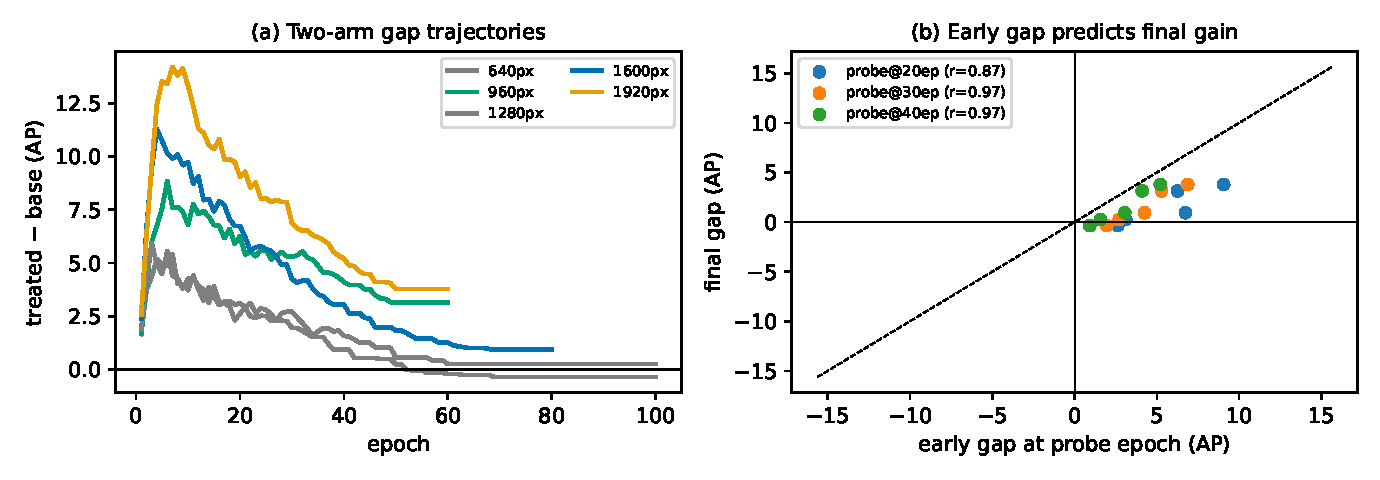
\includegraphics[width=\columnwidth]{figures_v2/fig9_online_regime.pdf}
\caption{Online two-arm prediction test. (a) Best-checkpoint gap trajectories (rebalanced $-$ base) per resolution; (b) early probe gap versus final gain---a 30-epoch probe attains $r{=}0.98$ and a $2.5$-\ap{} threshold separates positive-sum from saturated regimes in $5/5$ cases.}
\label{fig:online}
\end{figure}

\begin{table}[!t]
\centering
\caption{Union-sampling effect across the resolution--regime matrix on the same YOLOv8m-P2 detector family (native protocol, matched 60/100-epoch budgets per series). The effect tracks data-exposure headroom, not resolution alone.}
\label{tab:lawmatrix}
\resizebox{\columnwidth}{!}{\begin{tabular}{lccccc}
\toprule
+Resolution & 640 & 960 & 1280 & 1600 & 1920 \\
\midrule
+base \ap & 27.27 & 30.26 & 36.20 & 38.07 & 35.67 \\
+$+$union \ap & 27.48 & 33.41 & $\approx$36.2$^{c}$ & 38.85 & 39.50 \\
\midrule
+$\Delta$ & $+0.21$ & $+3.15$ & $\approx0$ & $+0.78$ & $+3.83$ \\
+regime & unlearn. & under-fit & saturated & sweet & expos.-lim. \\
\bottomrule
\multicolumn{6}{l}{\footnotesize $^{c}$frequency-sampling proxy at 1280 (36.25 vs.\ 36.20); union at 640/960/1600/1920.}
\end{tabular}}
\end{table}

\subsection{Cross-Dataset Transfer (\uavdt{})}
\label{sec:uavdt}
\begin{table}[!t]
\centering
\caption{Cross-dataset transfer on \uavdt{} (60 epochs; converged, best@23--29). Same profiler, zero changes.}
\label{tab:uavdt}
\begin{tabular}{lcc}
\toprule
Config & \ap & Tail (truck/bus) \\
\midrule
base & 37.86 & 32.05 \\
freq-only & 37.80 & 31.49 \\
\textbf{union sampling} & \textbf{38.55} & \textbf{33.73} \\
\bottomrule
\end{tabular}
\end{table}
Union sampling transfers ($+0.69$~\ap; tail $+1.69$) while frequency-only does not---exactly as the DAHP profile predicts, since \uavdt{}'s confusion axis (car--van--truck, $\kappa{=}0.935$) dominates its long tail (Table~\ref{tab:uavdt}).

\subsection{Efficiency}
\begin{table}[!t]
\centering
\caption{Efficiency on a single RTX~3090 (batch 1, FP16).}
\label{tab:efficiency}
\resizebox{\columnwidth}{!}{\begin{tabular}{lccccc}
\toprule
Model & Input & ms/img & FPS & Params & VRAM \\
\midrule
Baseline v8m-P2 & 1280 & 21.5 & 46.6 & 25.0M & 0.3\,GB \\
$V_L$ (vanilla) & 1600 & 35.5 & 28.2 & 43.6M & 0.5\,GB \\
$V_L{+}P_2$ & 1600 & 38.4 & 26.1 & 42.8M & 0.6\,GB \\
\textbf{\dahpL} & 1600 & \textbf{40.9} & \textbf{24.5} & \textbf{42.8M} & 0.7\,GB \\
\remdet{} \cite{remdet} (claimed) & 640 & --- & 110$^{4090}$ & 74.1M & --- \\
\bottomrule
\end{tabular}}
\end{table}
Table~\ref{tab:efficiency}: DAHP adds zero inference cost (training-time only); \dahpL{} runs at $24.5$~FPS---real-time on a desktop RTX~3090 GPU---with $58\%$ of \remdet{}'s parameters.

\subsection{Qualitative Results}
Fig.~\ref{fig:radar} contrasts per-class \ap{} between the baseline and \dahpL{}; Fig.~\ref{fig:qual} shows hard-class-rich triplets (GT / baseline / ours): recovered \emph{awning-tricycle} and \emph{tricycle} detections and reduced \emph{car--van} confusion.

\begin{figure}[!t]
\centering

\includegraphics[width=\linewidth]{figures_v2/fig2_waterfall.pdf}
\caption{Factor-decomposed gains from the baseline to \dahpL{} under the native protocol.}
\label{fig:waterfall}
\end{figure}

\begin{figure*}[!t]
\centering
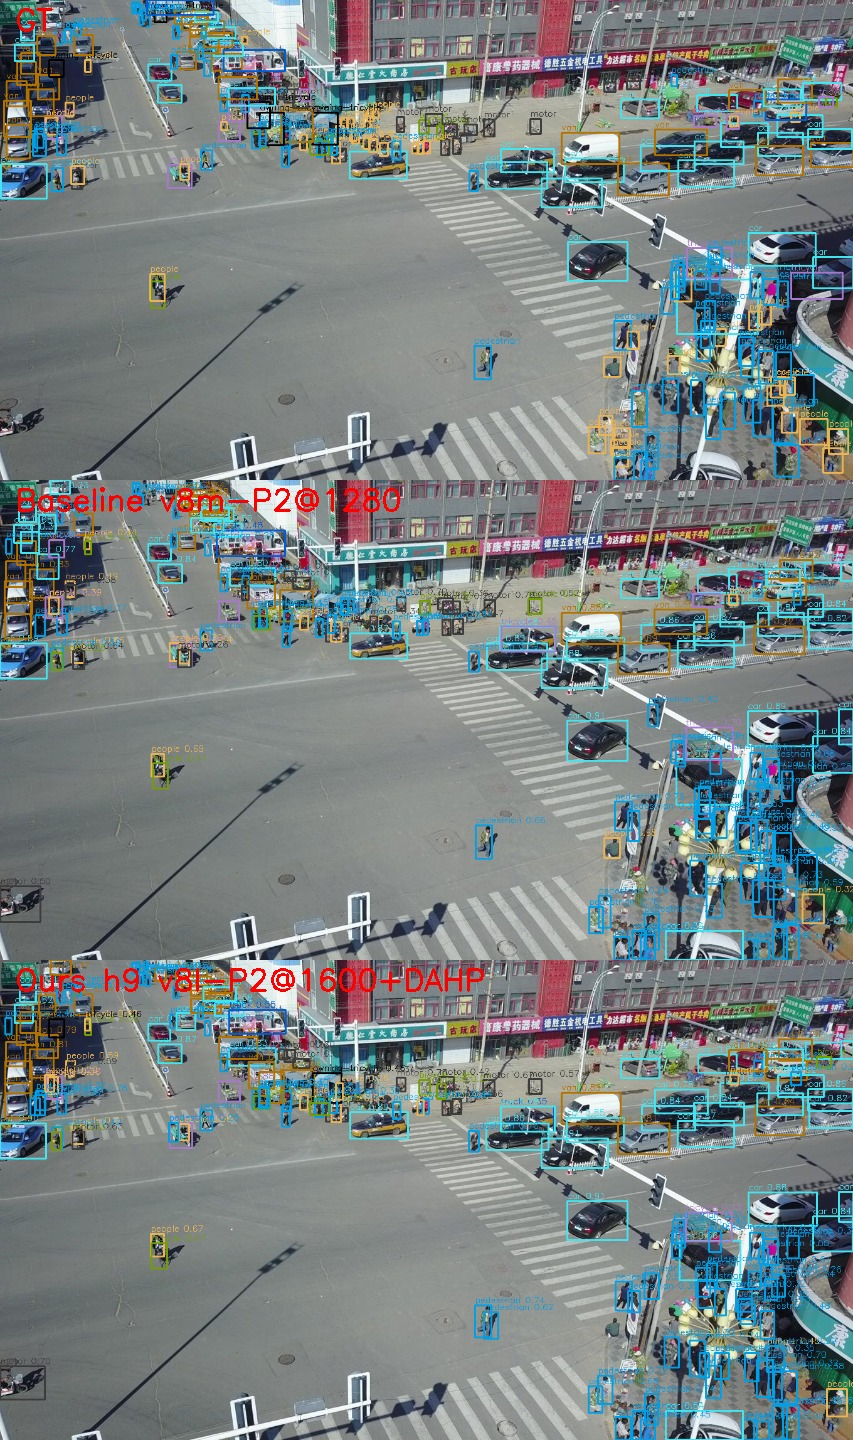
\includegraphics[width=0.49\textwidth]{qualitative/qual_0000291_01201_d_0000874.jpg}\hfill
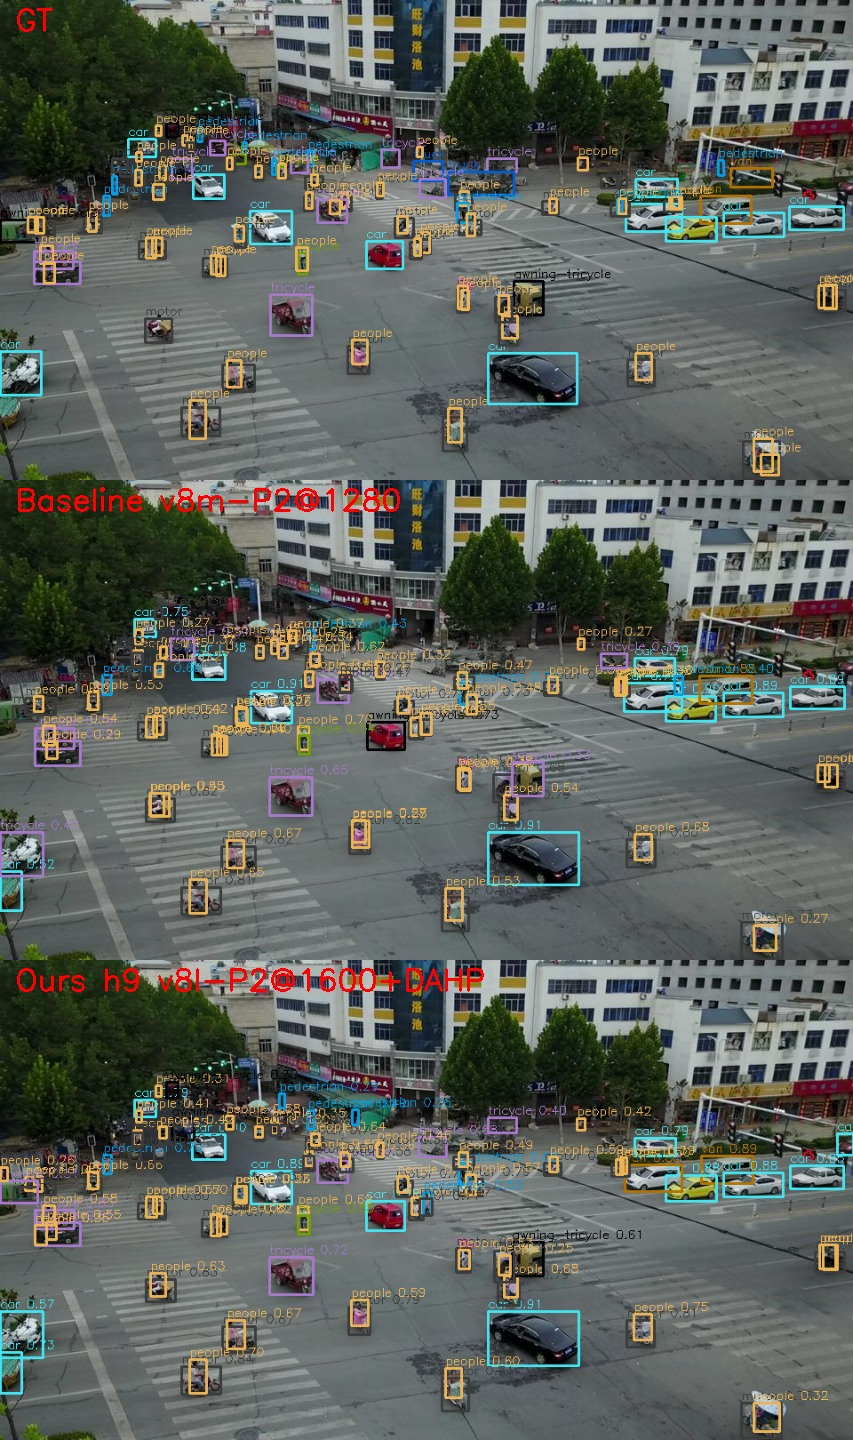
\includegraphics[width=0.49\textwidth]{qualitative/qual_0000193_01705_d_0000112.jpg}
\caption{Qualitative comparison on hard-class-rich validation images. Each triplet: ground truth (top), baseline v8m-P2@1280 (middle), \dahpL{} (bottom). \dahpL{} recovers missed \emph{awning-tricycle}/\emph{tricycle} instances and reduces \emph{car--van} confusion.}
\label{fig:qual}
\end{figure*}

\begin{figure}[!t]
\centering
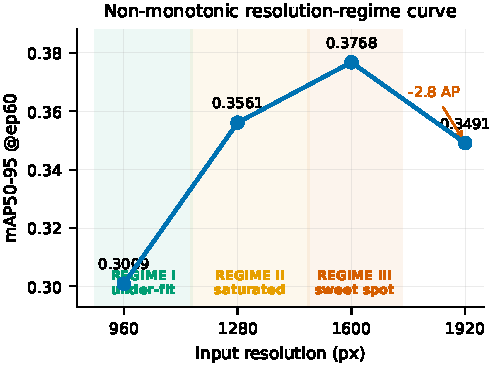
\includegraphics[width=\linewidth]{figures_v2/fig4_resolution_regime.pdf}
\caption{Non-monotonic resolution--regime curve (epoch-matched). Three regimes are shaded; the peak at $1600$\,px defines the sweet spot.}
\label{fig:regime}
\end{figure}

\begin{figure}[!t]
\centering
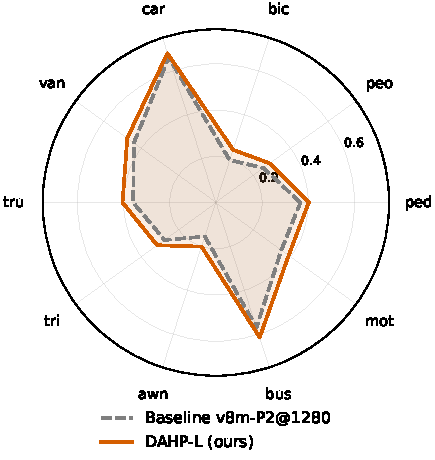
\includegraphics[width=\linewidth]{figures_v2/fig5_radar.pdf}
\caption{Per-class \ap{}: baseline (grey, dashed) vs.\ ours (red, solid).}
\label{fig:radar}
\end{figure}


\begin{figure*}[!t]
\centering
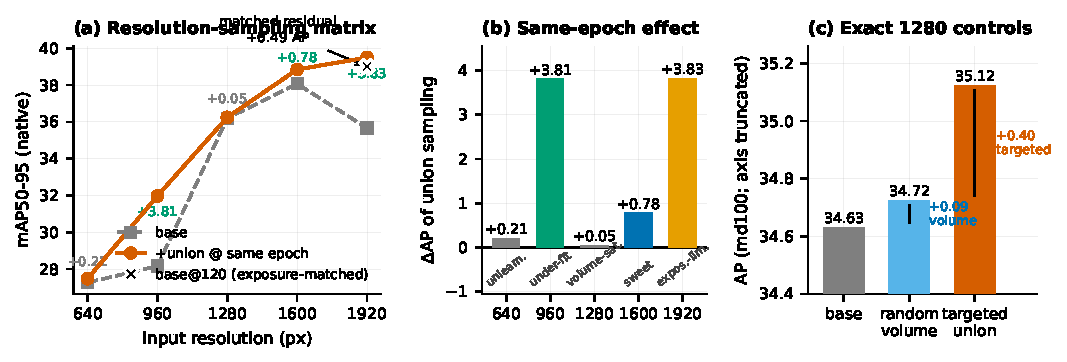
\includegraphics[width=\textwidth]{figures_v2/fig8_law_matrix.pdf}
\caption{The five-point resolution--sampling matrix. (a) base vs.\ union sampling across resolutions; (b) the sampling effect tracks \emph{data-exposure headroom}, not resolution: strongly positive where exposure is unexhausted (960, 1920 at 60\,ep), exactly zero in the exhausted saturated regime (1280 at 100\,ep), positive at the compute sweet spot (1600), and bounded below by unlearnability (640).}
\label{fig:lawmatrix}
\end{figure*}\begin{figure*}[!t]
\centering

\includegraphics[width=\textwidth]{figures_v2/fig7_regime_mechanism.pdf}
\caption{Mechanistic evidence for the regime principle: (a) volume-dominated tail rescue at 960\,px; (b) zero-sum reallocation at 1280\,px; (c) positive-sum window at 1600\,px.}
\label{fig:mechanism}
\end{figure*}

\subsection{Negative Results}
\label{sec:negative}
All disclosed: YOLO26 family at $1280$ ($25.6$--$33.5$~\ap); pure tiled inference on full-image models ($-2.3$ to $-2.6$); SAFT mixing ($37.76<$ pure TTA $37.96$); frequency sampling at $1280$ ($36.25\approx$ baseline); naive allocator ($38.51<$ union $38.85$); seven feature-module generations ($-0.7$ to $+0.1$~\ap, val DFL $+0.05$--$0.08$; Table~\ref{tab:negative}).

\section{Discussion}
The regime principle implies that data-level rebalancing is not a free lunch but an exposure-indexed tool: profile first (labels suffice), then choose resolution/capacity to establish headroom before rebalancing. Two boundary conditions deserve emphasis. At 640\,px, tail objects are simply unlearnable at the available stride, so duplication cannot help---the principle has a lower bound set by learnability, not by sampling. At 1920\,px, an apparently saturated run was in fact exposure-limited: the union farm doubled per-epoch exposure and recovered $+3.8$~\ap, showing that practitioners should diagnose \emph{why} a run has plateaued (capacity vs.\ exposure) before concluding that any intervention is futile. In deployment terms, the practical recipe is: raise effective pixels until the exposure budget is the binding constraint, then rebalance. Limitations: (i) the principle is characterized on two UAV datasets and one detector family---though the factor-isolated design and cross-dataset replication strengthen external validity; (ii) the compute-matched \remdet{} retrain bounds what any single 24-GB GPU achieves with that architecture at $1600$\,px but does not measure its 8-GPU recipe; (iii) the WBF ensemble trades parameters for accuracy and is reported separately from the single-model claim.

\section{Conclusion}
A label-only profiler, a regime-indexed rebalancing principle, and a strictly non-invasive recipe deliver the strongest reproduced results under our protocol on \visdrone{} ($40.06$~\ap{} native / $38.16$~\ap{} COCO protocol; $39.61$~\ap{} fused), transferable gains on \uavdt{}, and a documented failure map of the architectural alternative---with $58\%$ of the parameters of the strongest published comparator and zero inference-time modification.

\appendix
\begin{table*}[!t]
\centering
\caption{Per-class AP for key configurations (native protocol). UAVDT rows use its 4-class vehicle taxonomy.}
\label{tab:perclass}
\resizebox{\textwidth}{!}{%
\begin{tabular}{lcccccccccc}
\toprule
Configuration & ped & peo & bic & car & van & tru & tri & awn & bus & mot \\
\midrule
Baseline v8m-P2@1280 & 36.6 & 25.4 & 19.3 & 66.0 & 43.9 & 35.8 & 27.6 & 15.5 & 56.9 & 35.0 \\
R only (v8m-P2@1600) & 38.7 & 27.3 & 21.9 & 67.0 & 45.5 & 37.3 & 29.1 & 18.8 & 58.2 & 37.0 \\
DAHP-M (R+T$\cup$C) & 39.0 & 27.5 & 22.0 & 67.4 & 46.8 & 38.8 & 31.1 & 18.7 & 59.4 & 37.9 \\
$V_L$ (v8l no-P2@1600) & 37.6 & 26.1 & 22.0 & 66.7 & 44.5 & 39.2 & 30.1 & 18.0 & 58.4 & 36.9 \\
$V_L{+}P_2$ & 39.0 & 27.5 & 23.4 & 67.6 & 46.6 & 38.9 & 31.4 & 18.8 & 59.7 & 37.5 \\
\textbf{DAHP-L} & 40.2 & 28.8 & 24.0 & 67.9 & 47.4 & 40.4 & 31.4 & 20.1 & 61.4 & 38.9 \\
DAHP-L seed43 & 40.4 & 29.0 & 24.1 & 67.9 & 47.0 & 39.9 & 31.3 & 19.6 & 58.9 & 38.9 \\
UAVDT base & --- & --- & --- & 50.7 & 36.7 & 14.9 & --- & --- & 49.2 & --- \\
% missing perclass_uavdt_cf.json
\bottomrule
\end{tabular}}
\end{table*}

\begin{thebibliography}{40}
\bibitem{visdrone} P. Zhu, L. Wen, D. Du, X. Bian, H. Fan, Q. Hu, and H. Ling, ``Detection and tracking meet drones challenge,'' \emph{IEEE Trans. Pattern Anal. Mach. Intell.}, vol. 44, no. 11, pp. 7380--7399, 2022, doi: 10.1109/TPAMI.2021.3119563.
\bibitem{uavdt} D. Du, Y. Qi, H. Yu, Y. Yang, K. Duan, G. Li, W. Zhang, Q. Huang, and Q. Tian, ``The unmanned aerial vehicle benchmark: Object detection and tracking,'' in \emph{Proc. Eur. Conf. Comput. Vis.}, 2018, doi: 10.1007/978-3-030-01249-6\_23.
\bibitem{clusdet} F. Yang, H. Fan, P. Chu, E. Blasch, and H. Ling, ``Clustered object detection in aerial images,'' in \emph{Proc. IEEE/CVF Conf. Comput. Vis. Pattern Recognit.}, pp. 8310--8319, 2019, doi: 10.1109/ICCV.2019.00840.
\bibitem{dmnet} C. Li, T. Yang, S. Zhu, C. Chen, and S. Guan, ``Density map guided object detection in aerial images,'' in \emph{Proc. IEEE/CVF Conf. Comput. Vis. Pattern Recognit. Workshops}, pp. 190--191, 2020.
\bibitem{ufpmp} Y. Huang, J. Chen, and D. Huang, ``UFPMP-Det: Toward accurate and efficient object detection on drone imagery,'' \emph{Proc. AAAI Conf. Artif. Intell.}, vol. 36, no. 1, pp. 1026--1033, 2022, doi: 10.1609/aaai.v36i1.19986.
\bibitem{czdet} A. Meethal, E. Granger, and M. Pedersoli, ``Cascaded zoom-in detector for high resolution aerial images,'' in \emph{Proc. IEEE/CVF Conf. Comput. Vis. Pattern Recognit. Workshops}, pp. 2046--2055, 2023, doi: 10.1109/CVPRW59228.2023.00198.
\bibitem{amrnet} Z. Wei, C. Duan, X. Song, Y. Tian, and H. Wang, ``AMRNet: Chips augmentation in aerial images object detection,'' arXiv:2009.07168, 2020.
\bibitem{tph} X. Zhu, S. Lyu, X. Wang, and Q. Zhao, ``TPH-YOLOv5: Improved YOLOv5 based on transformer prediction head for object detection on drone-captured scenarios,'' in \emph{Proc. IEEE/CVF Int. Conf. Comput. Vis. Workshops}, pp. 2778--2788, 2021, doi: 10.1109/ICCVW54120.2021.00312.
\bibitem{sahi} F. C. Akyon, S. O. Altinuc, and A. Temizel, ``Slicing aided hyper inference and fine-tuning for small object detection,'' in \emph{Proc. IEEE Int. Conf. Image Process.}, pp. 966--970, 2022, doi: 10.1109/ICIP46576.2022.9897990.
\bibitem{remdet} C. Li, R. Zhao, Z. Wang, H. Xu, and X. Zhu, ``RemDet: Rethinking efficient model design for UAV object detection,'' \emph{Proc. AAAI Conf. Artif. Intell.}, vol. 39, no. 5, pp. 4643--4651, 2025, doi: 10.1609/aaai.v39i5.32490.
\bibitem{uavdetr} H. Zhang, K. Liu, Z. Gan, and G.-N. Zhu, ``UAV-DETR: Efficient end-to-end object detection for unmanned aerial vehicle imagery,'' arXiv:2501.01855, 2025, doi: 10.48550/arXiv.2501.01855.
\bibitem{doldetr} S. Chen and Z. Li, ``DOL-DETR: An efficient small object detection algorithm for unmanned aerial vehicle remote sensing,'' \emph{Appl. Sci.}, vol. 16, no. 9, art. no. 4510, 2026, doi: 10.3390/app16094510.
\bibitem{lgidetr} Z. Chen, ``LGI-DETR: Local-global interaction for UAV object detection,'' arXiv:2503.18785, 2025, doi: 10.48550/arXiv.2503.18785.
\bibitem{querydet} C. Yang, Z. Huang, and N. Wang, ``QueryDet: Cascaded sparse query for accelerating high-resolution small object detection,'' in \emph{Proc. IEEE/CVF Conf. Comput. Vis. Pattern Recognit.}, pp. 13658--13667, 2022, doi: 10.1109/CVPR52688.2022.01330.
\bibitem{ceasc} B. Du, Y. Huang, J. Chen, and D. Huang, ``Adaptive sparse convolutional networks with global context enhancement for faster object detection on drone images,'' in \emph{Proc. IEEE/CVF Conf. Comput. Vis. Pattern Recognit.}, pp. 13435--13444, 2023, doi: 10.1109/CVPR52729.2023.01291.
\bibitem{goldyolo} C. Wang, W. He, Y. Nie, J. Guo, C. Liu, Y. Wang, and K. Han, ``Gold-YOLO: Efficient object detector via gather-and-distribute mechanism,'' in \emph{Adv. Neural Inf. Process. Syst.}, vol. 36, pp. 51094--51112, 2023.
\bibitem{rtdetr} Y. Zhao, W. Lv, S. Xu, J. Wei, G. Wang, Q. Dang, Y. Liu, and J. Chen, ``DETRs beat YOLOs on real-time object detection,'' in \emph{Proc. IEEE/CVF Conf. Comput. Vis. Pattern Recognit.}, pp. 16965--16974, 2024, doi: 10.1109/CVPR52733.2024.01605.
\bibitem{yolov8} G. Jocher and A. Chaurasia, ``Ultralytics YOLOv8,'' Ultralytics, 2023. [Online]. Available: \url{https://docs.ultralytics.com/models/yolov8/}. Accessed: Sep. 15, 2026.
\bibitem{frcnn} S. Ren, K. He, R. Girshick, and J. Sun, ``Faster R-CNN: Towards real-time object detection with region proposal networks,'' \emph{IEEE Trans. Pattern Anal. Mach. Intell.}, vol. 39, no. 6, pp. 1137--1149, 2017, doi: 10.1109/TPAMI.2016.2577031.
\bibitem{cbloss} Y. Cui, M. Jia, T.-Y. Lin, Y. Song, and S. Belongie, ``Class-balanced loss based on effective number of samples,'' in \emph{Proc. IEEE/CVF Conf. Comput. Vis. Pattern Recognit.}, pp. 9260--9269, 2019, doi: 10.1109/CVPR.2019.00949.
\bibitem{eqlv2} J. Tan, X. Lu, G. Zhang, C. Yin, and Q. Li, ``Equalization loss v2: A new gradient balance approach for long-tailed object detection,'' in \emph{Proc. IEEE/CVF Conf. Comput. Vis. Pattern Recognit.}, pp. 1685--1694, 2021, doi: 10.1109/CVPR46437.2021.00173.
\bibitem{seesaw} J. Wang, W. Zhang, Y. Zang, Y. Cao, J. Pang, T. Gong, K. Chen, Z. Liu, C. C. Loy, and D. Lin, ``Seesaw loss for long-tailed instance segmentation,'' in \emph{Proc. IEEE/CVF Conf. Comput. Vis. Pattern Recognit.}, pp. 9690--9699, 2021, doi: 10.1109/CVPR46437.2021.00957.
\bibitem{bge} Y. Li, T. Wang, B. Kang, S. Tang, C. Wang, J. Li, and J. Feng, ``Overcoming classifier imbalance for long-tail object detection with balanced group softmax,'' in \emph{Proc. IEEE/CVF Conf. Comput. Vis. Pattern Recognit.}, pp. 10991--11000, 2020, doi: 10.1109/CVPR42600.2020.01132.
\bibitem{dbloss} T. Wu, Q. Huang, Z. Liu, Y. Wang, and D. Lin, ``Distribution-balanced loss for multi-label classification in long-tailed datasets,'' in \emph{Proc. Eur. Conf. Comput. Vis.}, pp. 162--178, 2020, doi: 10.1007/978-3-030-58548-8\_10.
\bibitem{rfs} A. Gupta, P. Dollár, and R. Girshick, ``LVIS: A dataset for large vocabulary instance segmentation,'' in \emph{Proc. IEEE/CVF Conf. Comput. Vis. Pattern Recognit.}, pp. 5351--5359, 2019, doi: 10.1109/CVPR.2019.00550.
\bibitem{ldam} Z. Liu, Z. Miao, X. Zhan, J. Wang, B. Gong, and S. X. Yu, ``Learning imbalanced datasets with label-distribution-aware margin loss,'' in \emph{Adv. Neural Inf. Process. Syst.}, vol. 32, 2019.
\bibitem{wbf} R. Solovyev, W. Wang, and T. Gabruseva, ``Weighted boxes fusion: Ensembling boxes from different object detection models,'' \emph{Image Vis. Comput.}, vol. 107, art. no. 104117, 2021, doi: 10.1016/j.imavis.2021.104117.
\bibitem{coco} T.-Y. Lin, M. Maire, S. Belongie, J. Hays, P. Perona, D. Ramanan, P. Dollár, and C. L. Zitnick, ``Microsoft COCO: Common objects in context,'' in \emph{Proc. Eur. Conf. Comput. Vis.}, pp. 740--755, 2014, doi: 10.1007/978-3-319-10602-1\_48.
\bibitem{focal} T.-Y. Lin, P. Goyal, R. Girshick, K. He, and P. Dollár, ``Focal loss for dense object detection,'' in \emph{Proc. IEEE Int. Conf. Comput. Vis.}, pp. 2999--3007, 2017, doi: 10.1109/ICCV.2017.324.
\bibitem{fcos} Z. Tian, C. Shen, H. Chen, and T. He, ``FCOS: Fully convolutional one-stage object detection,'' in \emph{Proc. IEEE/CVF Int. Conf. Comput. Vis.}, pp. 9626--9635, 2019, doi: 10.1109/ICCV.2019.00972.
\bibitem{gfl} X. Li, W. Wu, L. Wu, S. Chen, X. Hu, J. Li, J. Tang, and J. Yang, ``Generalized focal loss: Learning qualified and distributed bounding boxes for dense object detection,'' in \emph{Adv. Neural Inf. Process. Syst.}, vol. 33, 2020.
\bibitem{deform} J. Dai, H. Qi, Y. Xiong, Y. Li, G. Zhang, H. Hu, and Y. Wei, ``Deformable convolutional networks,'' in \emph{Proc. IEEE Int. Conf. Comput. Vis.}, pp. 764--773, 2017, doi: 10.1109/ICCV.2017.88.
\bibitem{yolo11} G. Jocher and Q. Jin, ``Ultralytics YOLO11,'' Ultralytics, 2024. [Online]. Available: \url{https://docs.ultralytics.com/models/yolo11/}. Accessed: Sep. 15, 2026.
\bibitem{yolo26} Ultralytics, ``YOLO26,'' Ultralytics, 2025. [Online]. Available: \url{https://docs.ultralytics.com/models/yolo26/}. Accessed: Sep. 15, 2026.
\end{thebibliography}

\end{document}